\documentclass{beamer}
  % Beamer settings
  \usetheme{Berkeley}
  \usecolortheme{dove}
  \usecolortheme{rose}
  \usefonttheme{professionalfonts}
  \usefonttheme{serif}
  \setbeamertemplate{bibliography item}{}

  % Packages and settings
  \usepackage{fontspec}
    \setmainfont{Charis SIL}
  \usepackage[normalem]{ulem}
  \usepackage{pifont}
  \usepackage{hyperref}
    \hypersetup{colorlinks=true,
                allcolors=blue}
  \usepackage{graphicx}
    \graphicspath{{./figure/}}
  \usepackage[backend=biber, style=apa]{biblatex}
    \addbibresource{../ling_intro/references/References.bib}
  \usepackage{tikz}
    \usetikzlibrary{shapes.geometric, arrows, positioning}
    \tikzstyle{box} = [rectangle,
                       text centered,
                       draw=black,
                       align=center]
    \tikzstyle{heading} = [rectangle,
                           text centered,
                           draw=none,
                           align=center]
    \tikzstyle{arrow} = [thick,->]
  \usepackage{adjustbox}

  % Document information
  \author{Joshua McNeill}
  \title{Le français \sout{en} dans la Louisiane}
  \institute{\url{joshua.mcneill@uga.edu}}
  \date{28 avril 2022}

  % New commands
  \newcommand{\xmark}{\textcolor{red}{\ding{56}}}

\begin{document}
  % Intro stuff
  \begin{frame}
    \titlepage
  \end{frame}
  \begin{frame}
    \tableofcontents[hideallsubsections]
  \end{frame}
  \AtBeginSection[]{
    \begin{frame}
      \tableofcontents[currentsection,
                       hideallsubsections]
    \end{frame}
  }

  % Meat and potatoes
  \section{Le sud de la Louisiane}
    \begin{frame}{}
      Arakansas du sud $\downarrow$
      \begin{columns}
        \column{0.63\textwidth}
          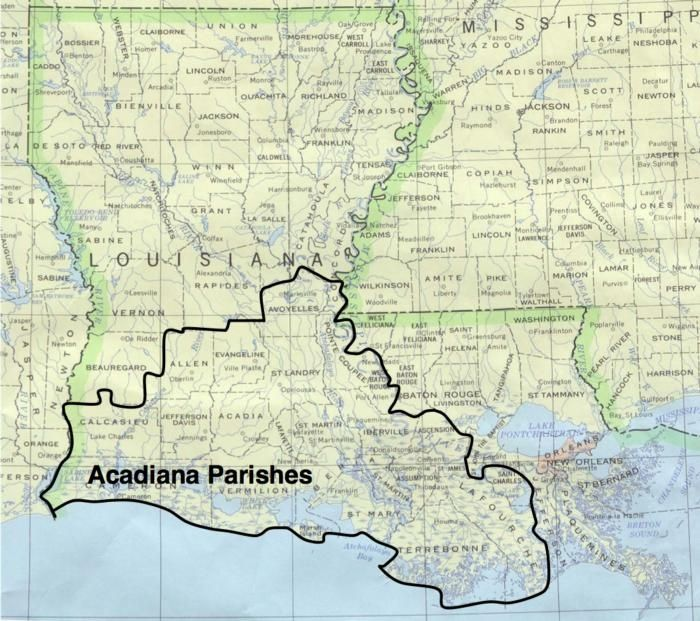
\includegraphics[scale=0.27]{acadiana.jpg}
        \column{0.36\textwidth}
          \begin{minipage}[0.6\textheight]{\linewidth}
            \only<1>{
              \rule{0pt}{70pt}
              Nouvelle-Orléans \\
              $\leftarrow$
            }
            \only<2->{
              Contrôle
              \begin{enumerate}
                \item France (1682-1760)
                \item Espagne (1760-1800)
                \item France (1800-1803)
                \item É.-U. (1803-présent)
              \end{enumerate}
            }
          \end{minipage}
      \end{columns}
      Louisiane du sud $\uparrow$ \\
    \end{frame}

    \begin{frame}{}
      \begin{columns}
        \column{0.6\textwidth}
          \begin{center}
            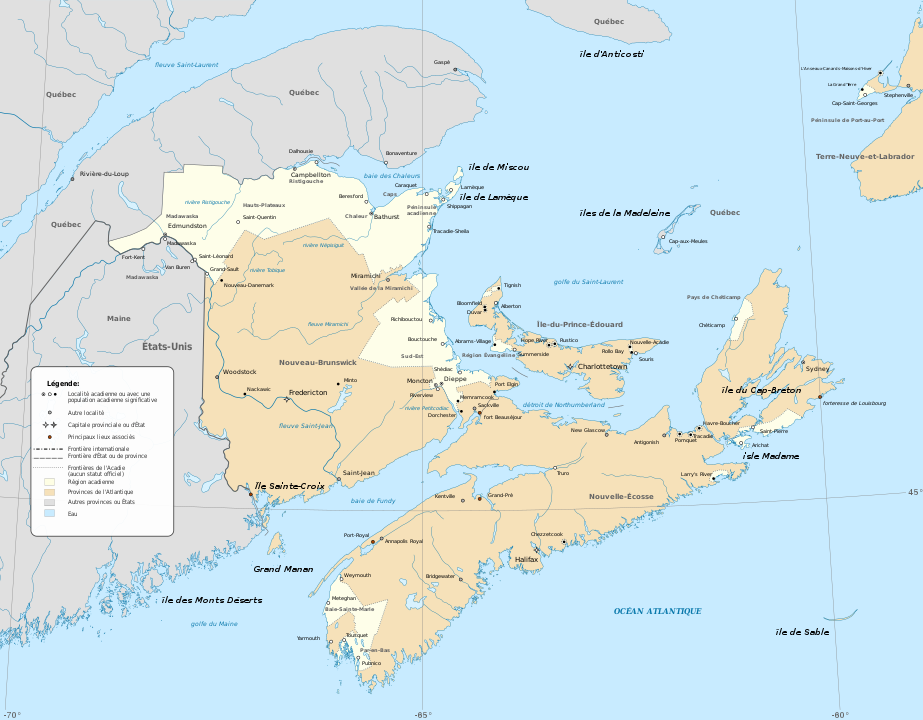
\includegraphics[scale=0.15]{acadie.png}
          \end{center}
          \begin{columns}
            \column{0.5\textwidth}
              \includegraphics[scale=0.11]{îles_canaries.png}
            \column{0.5\textwidth}
              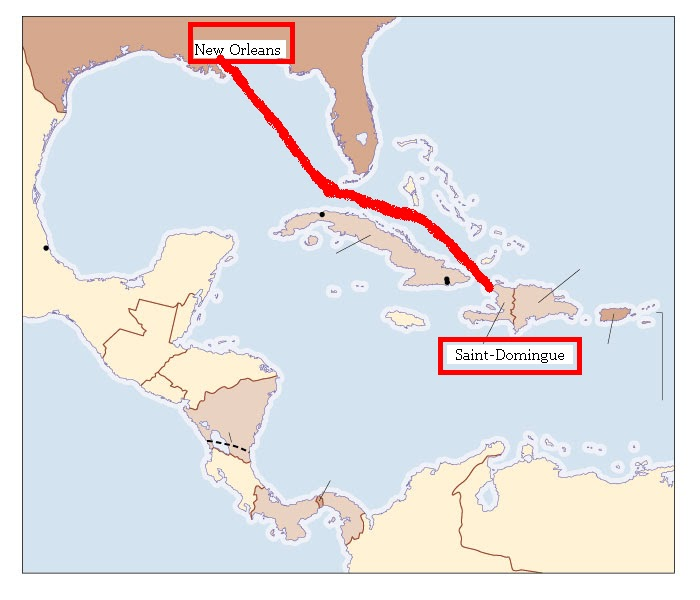
\includegraphics[scale=0.14]{saint-domingue.jpg}
          \end{columns}
        \column{0.39\textwidth}
          Immigration
          \begin{enumerate}
            \item Acadie (1760)
            \item Îles Canaries (1778)
            \item Saint-Domingue (1800)
          \end{enumerate}
      \end{columns}
    \end{frame}
  \section{Les Cadiens et les Créoles}
    \begin{frame}{}
      \begin{columns}
        \column{0.49\textwidth}
          % \begin{minipage}[0.6\textheight]{\linewidth}
            Les Cadiens
            \begin{enumerate}
              \item Ruraux
              \item Isolés
              \item Catholiques
              \item Francophones
              \item Ancêtres acadiens
            \end{enumerate}
          % \end{minipage}
        \column{0.49\textwidth}
          % \only<1>{
          %   \includegraphics[scale=0.07]{cléoma.jpg}
          % }
          % \only<2->{
            \href{https://youtu.be/hkophR-j0SU}{
              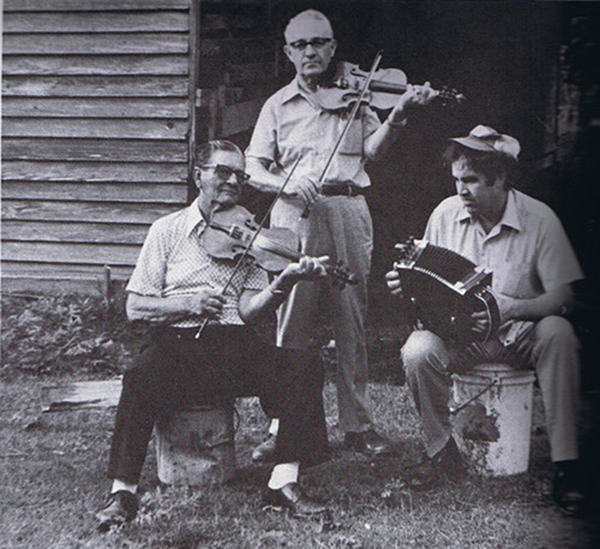
\includegraphics[scale=0.17]{dennis_mcgee.jpg}
            }
          % }
      \end{columns}
    \end{frame}

    \begin{frame}{}
      \begin{columns}
        \column{0.49\textwidth}
          \begin{minipage}[0.6\textheight]{\linewidth}
            Les Créoles \\
            \only<1>{(à la période coloniale)}\only<2>{(au 19e siècle)}\only<3->{(au 20e siècle)}
            \begin{enumerate}
              \item \only<1>{Européens (français ou espagnols)} \only<2->{\sout{Européens (français ou espagnols)}}
              \item Nés en Louisiane
              \uncover<2->{
                \item \only<2>{Gens de couleur libres} \only<3->{\sout{Gens de couleur libres}}
              }
              \uncover<3->{
                \item Noirs
                \item Francophones ou créolophones
              }
            \end{enumerate}
          \end{minipage}
        \column{0.49\textwidth}
          \only<1>{
            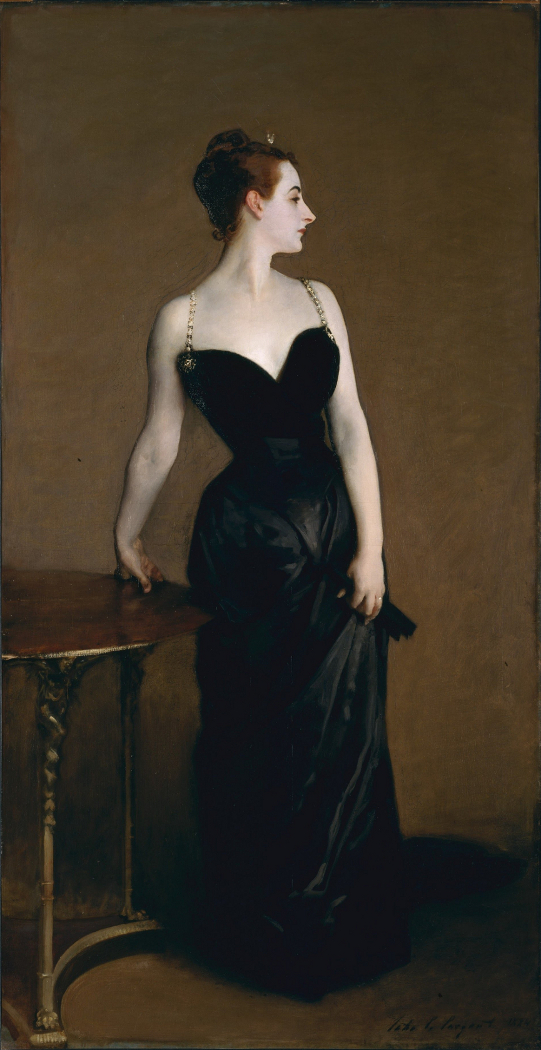
\includegraphics[scale=0.175]{madame_x.jpg}
          }
          \only<2>{
            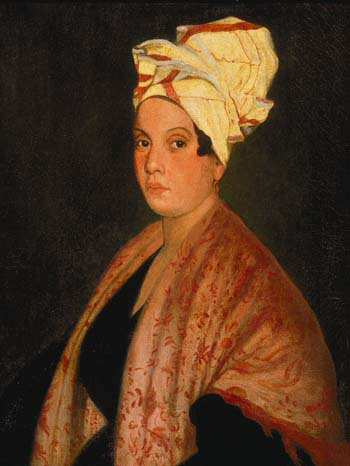
\includegraphics[scale=0.25]{laveau.png}
          }
          \only<3->{
            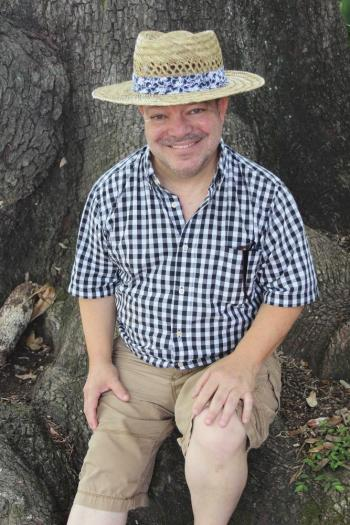
\includegraphics[scale=0.3]{lafleur.jpg}
          }
      \end{columns}
    \end{frame}

    \begin{frame}{}
      \begin{center}
        
\includegraphics[scale=0.09]{codofil.jpg} \\
        \hrule
        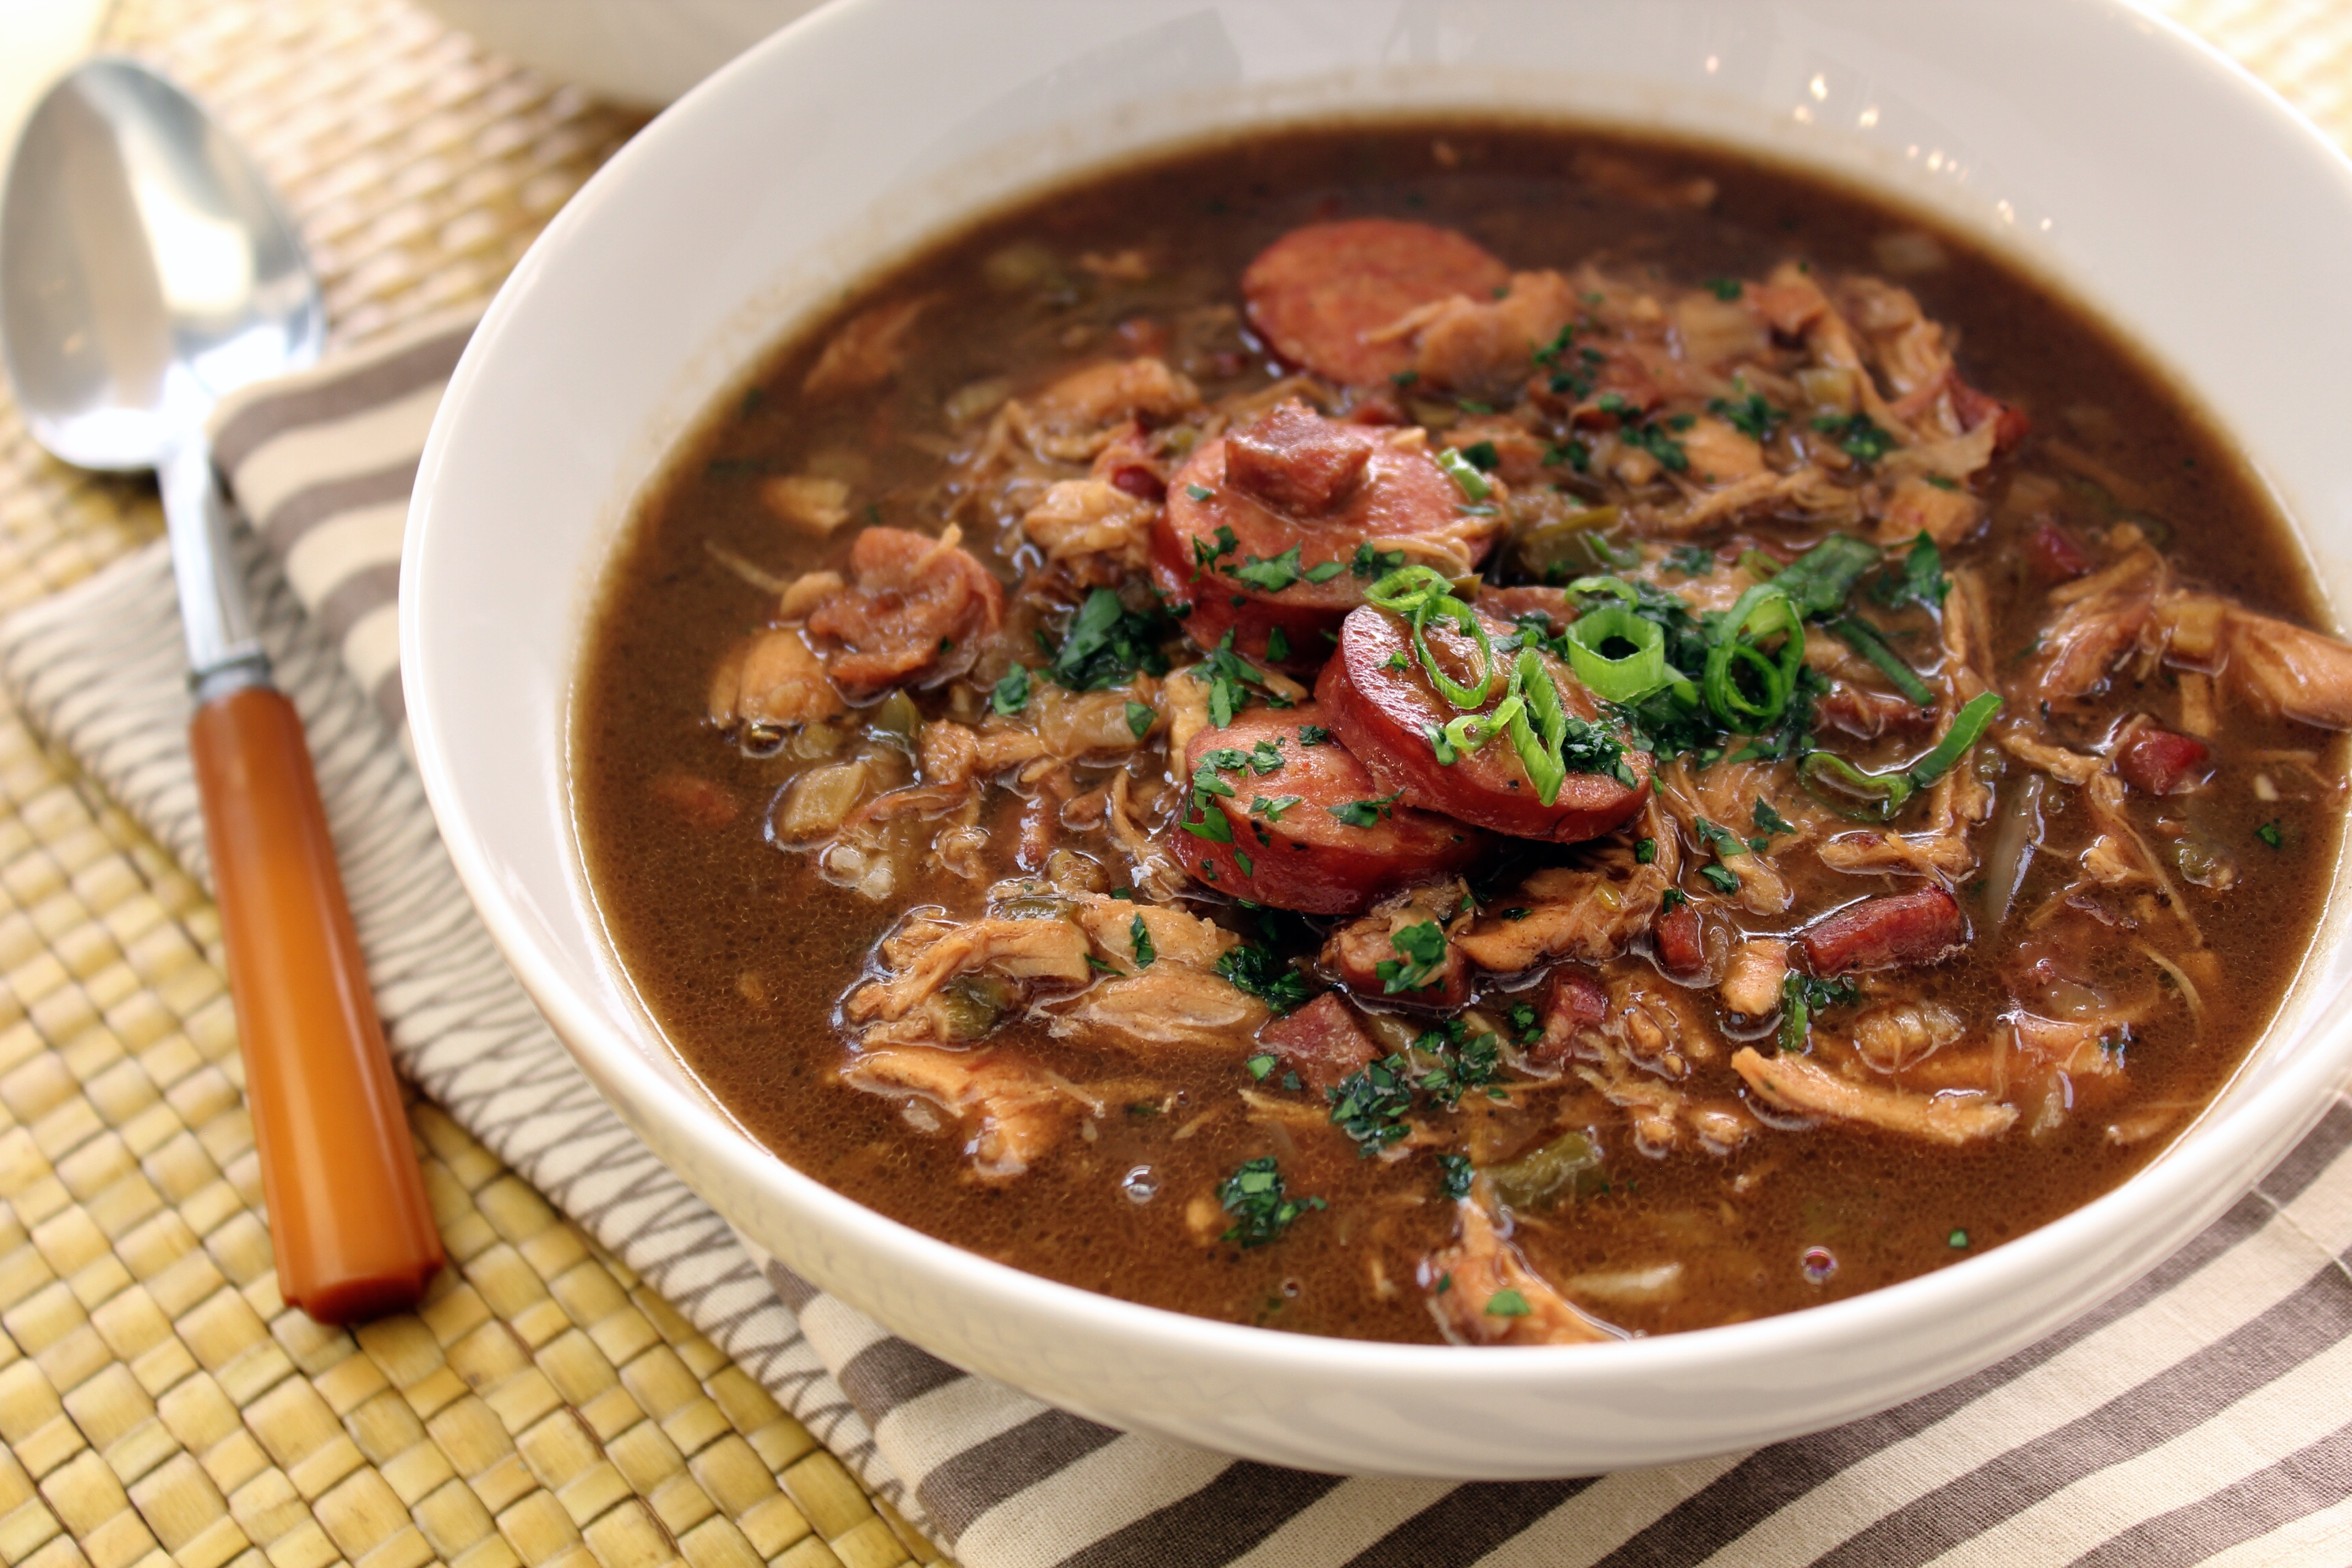
\includegraphics[scale=0.025]{gumbo.jpg}
        
\includegraphics[scale=0.105]{bojangles_cajun.jpg}
        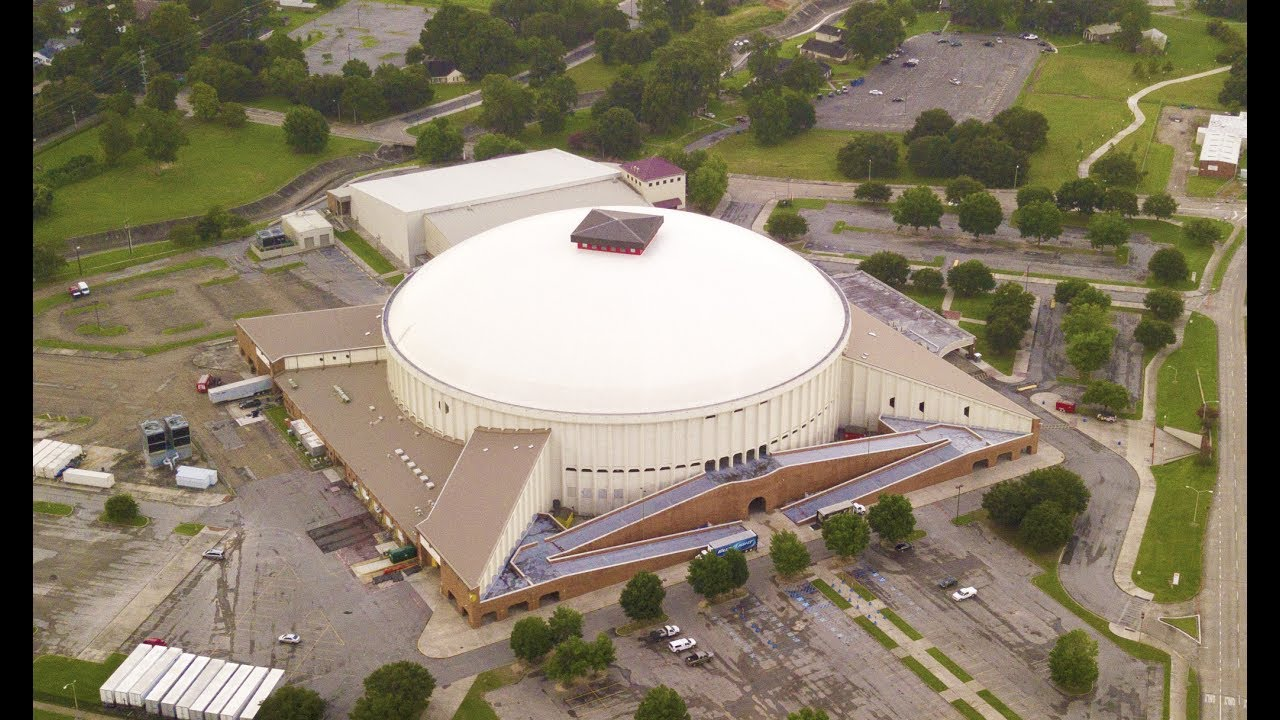
\includegraphics[scale=0.08]{cajundome.jpg}
      \end{center}
    \end{frame}
  \section{Le français \sout{cadien} louisianais}
    \begin{frame}{}
      \begin{adjustbox}{width=0.98\textwidth}
        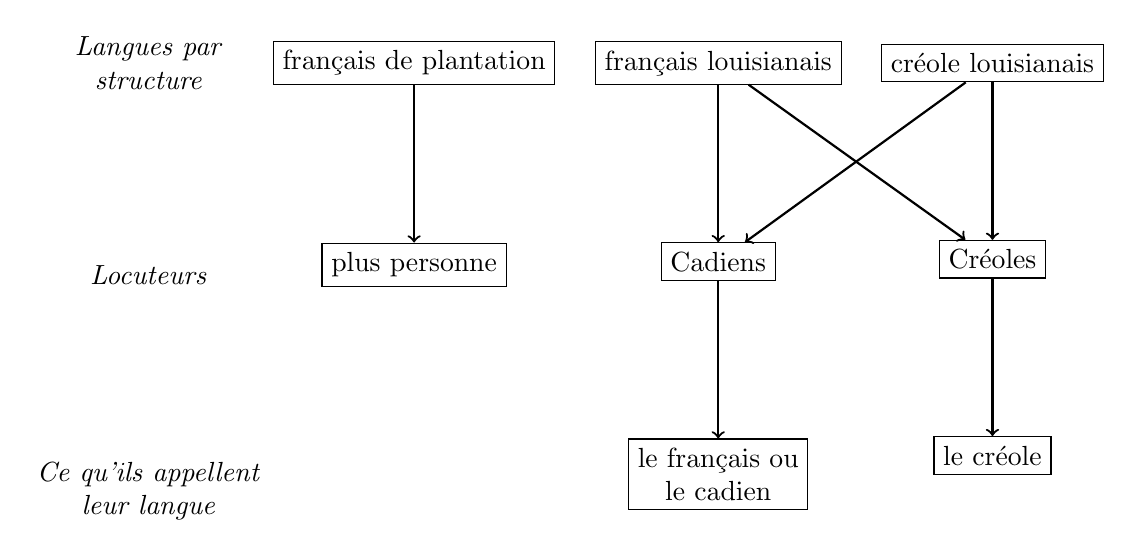
\begin{tikzpicture}
          \node (langues)    [heading]                         {\emph{Langues par}\\
                                                                \emph{structure}};
          \node (plantation) [box, right=0.5cm of langues]     {français de plantation};
          \node (français)   [box, right=0.5cm of plantation]  {français louisianais};
          \node (créoleStr)  [box, right=0.5cm of français]    {créole louisianais};
          \node (locuteurs)  [heading, below=2cm of langues]   {\emph{Locuteurs}};
          \node (personne)   [box, below=2cm of plantation]    {plus personne};
          \node (cadiens)    [box, below=2cm of français]      {Cadiens};
          \node (créoles)    [box, below=2cm of créoleStr]     {Créoles};
          \node (nom)        [heading, below=2cm of locuteurs] {\emph{Ce qu'ils appellent}\\
                                                                \emph{leur langue}};
          \node (cadien)     [box, below=2cm of cadiens]       {le français ou\\
                                                                le cadien};
          \node (créoleL)    [box, below=2cm of créoles]       {le créole};
          \draw [arrow] (plantation) -- (personne);
          \draw [arrow] (français)   -- (cadiens);
          \draw [arrow] (français)   -- (créoles);
          \draw [arrow] (créoleStr)  -- (cadiens);
          \draw [arrow] (créoleStr)  -- (créoles);
          \draw [arrow] (cadiens)    -- (cadien);
          \draw [arrow] (créoles)    -- (créoleL);
        \end{tikzpicture}
      \end{adjustbox}
    \end{frame}

    \begin{frame}[t]{}
      \centering
      \href{https://youtu.be/2Xs_9rEh1Ec?t=136}{Canray Fontenot, musicien}
      \begin{columns}
        \column{0.48\textwidth}
          \centering
          Le français
        \column{0.48\textwidth}
          \centering
          Le créole
      \end{columns}
    \end{frame}

    \begin{frame}[t]{}
      \centering
      \href{https://youtu.be/6hf5PUe2TSA?t=97}{Hermean Dunbar}
      \begin{columns}
        \column{0.48\textwidth}
          \centering
          Le français
        \column{0.48\textwidth}
          \centering
          Le créole
      \end{columns}
    \end{frame}

    \begin{frame}[t]{}
      \centering
      \href{https://youtu.be/siflvTt24Zw?t=121}{Nathan Rabalais, professeur}
      \begin{columns}
        \column{0.48\textwidth}
          \centering
          Le français
        \column{0.48\textwidth}
          \centering
          Le créole
      \end{columns}
    \end{frame}

    \begin{frame}[t]{}
      \centering
      \href{https://youtu.be/-lgXc_-a9Kc?t=99}{Rose Begnaud Tessier}
      \begin{columns}
        \column{0.48\textwidth}
          \centering
          Le français
        \column{0.48\textwidth}
          \centering
          Le créole
      \end{columns}
    \end{frame}

    \begin{frame}[t]{}
      \centering
      \href{https://youtu.be/QodpvU-Z2PI?t=83}{Des traductions}
      \begin{columns}
        \column{0.48\textwidth}
          \centering
          Le français
        \column{0.48\textwidth}
          \centering
          Le créole
      \end{columns}
    \end{frame}

    \begin{frame}[t]{}
      \centering
      \href{https://youtu.be/Xj_AtDj-LT4?t=87}{Liz Huval}
      \begin{columns}
        \column{0.48\textwidth}
          \centering
          Le français
        \column{0.48\textwidth}
          \centering
          Le créole
      \end{columns}
    \end{frame}

    \begin{frame}[t]{}
      \centering
      \href{https://youtu.be/OHNR8ZTPBmQ?t=150}{Theresa Dardar}
      \begin{columns}
        \column{0.48\textwidth}
          \centering
          Le français
        \column{0.48\textwidth}
          \centering
          Le créole
      \end{columns}
    \end{frame}
\end{document}
